\documentclass[usenames,dvipsnames]{beamer}
\usetheme{default}

\usepackage{amsmath}
\usepackage{amssymb}
\usepackage{amsfonts}
\usepackage{listings}

\renewcommand{\iff}{\Leftrightarrow}
\renewcommand{\implies}{\Rightarrow}
\newcommand{\pointsto}{\hookrightarrow}
\newcommand{\reach}[2]{\mathrm{reach}\left(#1, #2\right)}
\newcommand{\markset}[2]{\mathrm{mark}\left(#1, #2\right)}
\newcommand{\id}{\mathrm{id}}
\newcommand{\gchead}[1]{\mathrm{gchead}\left(#1\right)}
\newcommand{\free}[1]{\mathrm{free}\left(#1\right)}
\newcommand{\marked}[2]{\mathrm{marked}\left(#1, #2\right)}
\newcommand{\type}[1]{\mathrm{type}\left(#1\right)}
\newcommand{\typointer}{\mathrm{pointer}}

\definecolor{LightGray}{rgb}{0.9,0.9,0.9}

\lstset{basicstyle=\footnotesize\ttfamily}
\lstset{showstringspaces=false}
\lstset{numbers=none}
\lstset{keywordstyle=\color{MidnightBlue}\bfseries}
\lstset{commentstyle=\color{JungleGreen}}
\lstset{identifierstyle=\color{OliveGreen}}
\lstset{stringstyle=\color{Red}}
\lstset{backgroundcolor=\color{LightGray}}
\lstset{breaklines=true}
\lstset{captionpos=b}

\author{Michael Walker}
\title{A verified memory-management system for dynamic languages}
\institute{Department of Computer Science\\
  University of York\\
  \texttt{msw504@york.ac.uk}
}

\begin{document}

\begin{frame}[plain]
  \only<1>{\titlepage}

  % Hello, I'm Michael Walker, and my project was originally entitled
  % "A verified memory-management system for dynamic languages", but
  % it actually ended up just being about

  \only<2>{\centering \huge Verified Garbage Collection}

  % verified garbage collection in general.
\end{frame}

\begin{frame}{Overview}
  \tableofcontents

  % So I'll start by giving the motivation, and quickly introducing
  % the topics of garbage collection and software verification; and
  % then I'll go through what I did in this project: specifically,
  % determining what it means for various types of garbage collector
  % to be correct, looking at existing collectors as case studies, and
  % then generalising to produce a more widely-applicable definition
  % of correctness; and I'll conclude by evaluating the work, and just
  % briefly summarising the contributions again.
\end{frame}

%% Introduction

\section{Introduction}
\subsection{Motivation}

\begin{frame}{Motivation}
  \begin{itemize}
  \item Memory bugs can produce incorrect program results.
    \begin{itemize}
    \item The recent Heartbleed exploit in OpenSSL is a good (or bad)
      example of this.
    \end{itemize}
  \item Can be hard to track down by hand.
  \item \textit{``testing shows the presence, not the absence of
      bugs''}
  \item Typically no formal verification, only testing.
  \end{itemize}

% Memory is hard to get right, and getting it wrong can have dire
% consequences. The recent Heartbleed exploit in OpenSSL is a good
% example of this. That wasn't a garbage collection problem, but it
% did arise from a hard-to-find bug in an unverified memory management
% system.

% In a garbage collected program, the sorts of errors that could arise
% include freeing some memory whilst it is still needed, which could
% in the best case result in a crash, and the worst case an incorrect
% computation. However, it's easier to trust a garbage collector than
% it is to handle all of your memory yourself, and so garbage
% collectors have become a staple feature of modern programming
% languages, freeing the programmer to worry about more high-level
% concerns.

% Because memory is hard to get right, memory managers, like garbage
% collectors, tend to be complex, and it's often difficult to be sure
% they're right. Because of this, testing is widely used, but this
% isn't enough to guarantee correctness. The only way to be sure that
% there are no bugs is to construct a proof that the collector does do
% what it is supposed to do.
\end{frame}

\subsection{Garbage Collection}

\begin{frame}{Garbage Collection}
  \only<1>{
    \begin{figure}[h!]
      \centering
      \includegraphics{../csw/heap1}
      \label{fig:heap1}
      \caption{No garbage: $A$ and $B$ reachable from the roots}
    \end{figure}
  }

% Garbage collection is the process of automatically removing
% unreachable memory from the heap, decreasing the memory usage of a
% program. If we consider the heap to be a digraph of memory cells
% connected by pointers, then the roots of this structure are the
% variables which are currently in scope: the stack.

  \only<2>{
    \begin{figure}[h!]
      \centering
      \includegraphics{../csw/heap2}
      \label{fig:heap2}
      \caption{$A$ becomes garbage when one of the roots is changed to
        point at $B$.}
    \end{figure}
  }

% A cell might become garbage when roots change, or when another cell
% is mutated. If a cell is garbage, it's useless. We don't want it any
% more. We'd much rather reduce the heap to

  \only<3>{
    \begin{figure}[h!]
      \centering
      \includegraphics{../csw/heap3}
      \label{fig:heap3}
      \caption{Remove $A$, so the heap is now minimal.}
    \end{figure}
  }

% this, as it's smaller.
\end{frame}

\begin{frame}{Garbage Collection: Mark-Sweep and Copying}
  \begin{figure}[h]
    \centering
    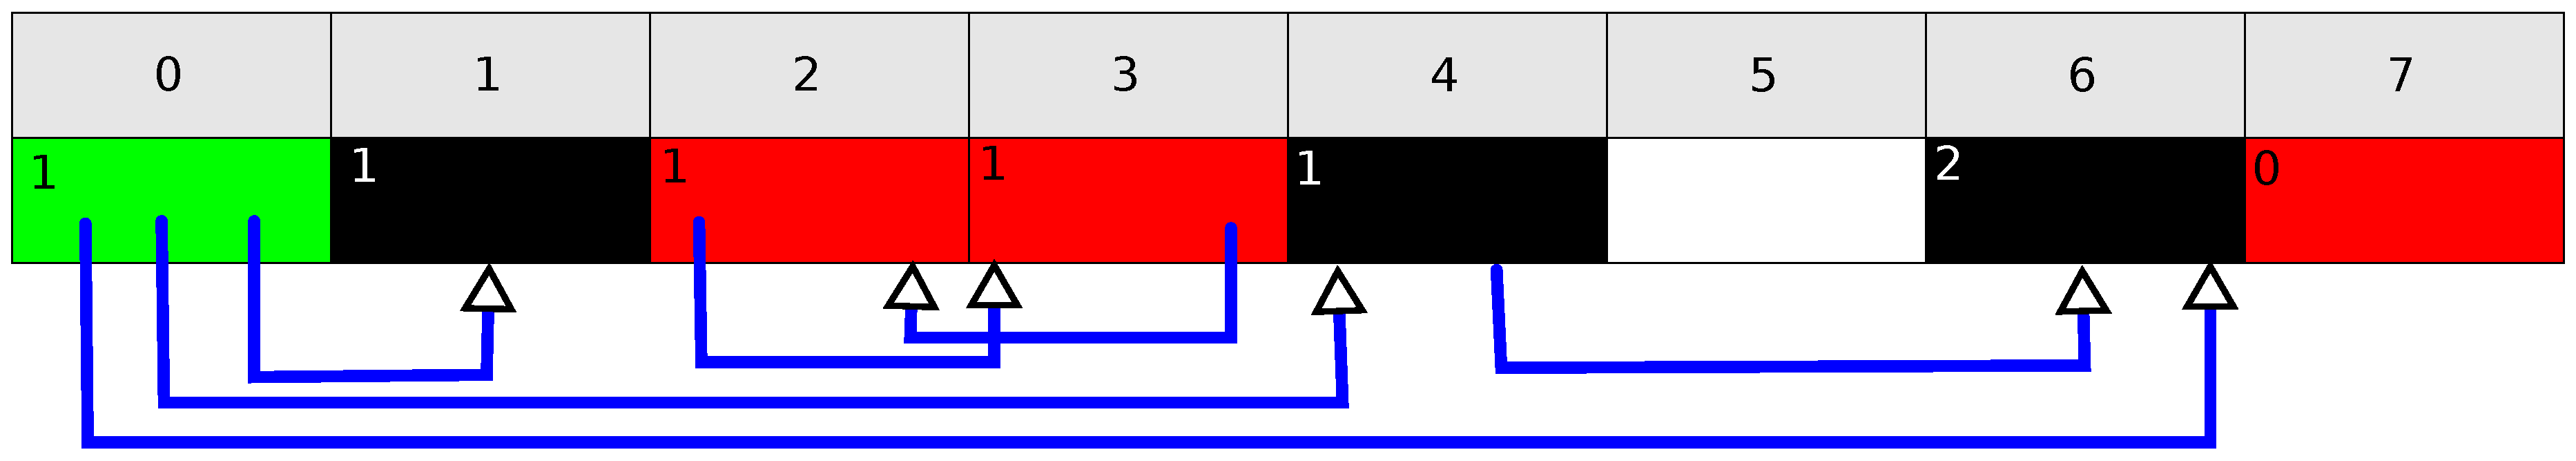
\includegraphics[width=\textwidth]{../../dissertation/lit-gc-before}
    \caption{Heap before garbage collection}
    \label{fig:lit-gc-before}
  \end{figure}

% I'll be using a little example to explain the two types of garbage
% collector I considered: green cells are live, red are garbage, and
% white are free.

  \only<2>{
    \begin{figure}[h]
      \centering
      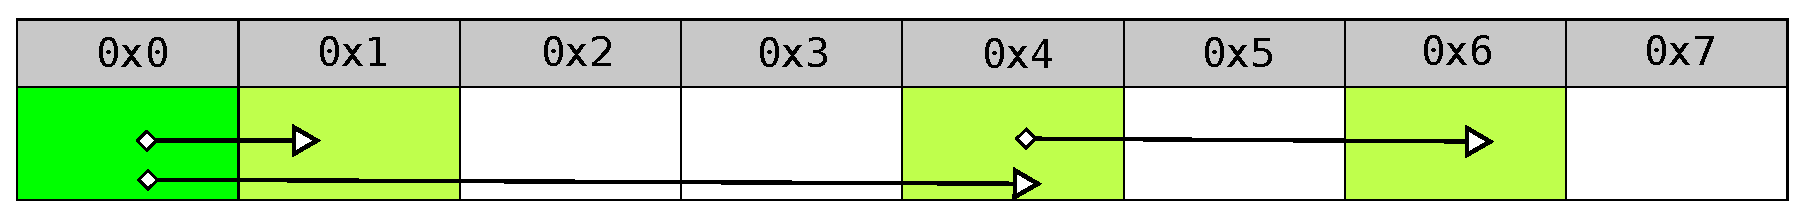
\includegraphics[width=\textwidth]{../../dissertation/lit-gc-marksweep}
      \caption{Heap after mark-sweep collection}
      \label{fig:lit-gc-marksweep}
    \end{figure}

    \begin{itemize}
    \item Cells have a ``mark bit'', initially unset
    \item Heap is traversed from roots, setting mark bits (marking)
    \item Heap is traversed totally, freeing unmarked cells (sweeping)
    \item Removes all garbage
    \item Takes time proportional to the size of the heap
    \end{itemize}
  }

% Mark-sweep collectors date from the early days of Lisp, and work by
% assigning to every cell a mark bit, which is initially unset. Upon
% running out of memory, the heap is traversed from the roots, and
% every cell reached has the mark bit set. Then the heap is traversed
% again, but this time the entire heap is traversed, and all marked
% cells are unmarked, and all unmarked cells are freed. This gets rid
% of all garbage, it's nice and simple to implement, but takes time
% proportional to the size of the heap, regardless of how many cells
% actually survive.

  \only<3>{
    \begin{figure}[h]
      \centering
      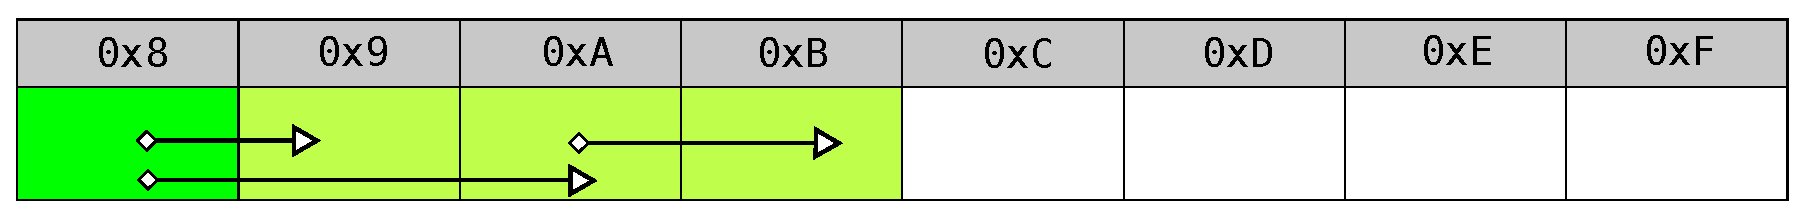
\includegraphics[width=\textwidth]{../../dissertation/lit-gc-copying}
      \caption{Heap after copying collection}
      \label{fig:lit-gc-copying}
    \end{figure}

    \begin{itemize}
    \item Divides heap into two ``semispaces''
    \item Allocation only happens in one at a time
    \item At GC, live cells are copied to the other space, and the
      roles swapped
    \item Takes time proportional to size of the live portion of the
      heap
    \item Has a space cost of half the heap
    \item Potentially reduces cache misses and page faults.
    \end{itemize}
  }

% Copying collectors are pretty different, they work by dividing the
% heap into two equal-sized pieces, in only one of which allocation
% happens. Upon running out of memory the heap is traversed from the
% roots, and all cells reached are copied to the other space and
% pointers updated, then allocation switches to happening in that
% space. This only takes time proportional to the size of the live
% portion of the heap, but it has a large space cost. However, by
% compacting the heap it improves locality of reference, and so can
% potentially have a side effect of reducing cache misses and page
% faults.
\end{frame}

\subsection{Software Verification}

\begin{frame}{Software Verification}
  \begin{itemize}
  \item Produce a formal model from some code.
  \item Produce a formal model from a specification.
  \item Reason about the relation between the two.
  \end{itemize}

% Briefly, the idea behind software verification is that when you
% write some software, or at least the sort of software which you
% might want to verify, you don't just start going. You first produce
% a specification. Then, when you're done, you want to be sure that
% the code and the specification are actually talking about the same
% thing, but they're on totally different levels of abstraction, which
% complicates this. So what you do is you produce a formal model of
% how the code works, usually in terms of how it manipulates the
% program state, and a formal model of what the specification
% describes, and then use some logic to reason about the two.

% There's a slightly different way of approaching this, where you
% instead start from the formal specification, and keep producing
% slightly lower-level specifications until you get to code. If you
% have an unbroken chain of proofs, then by transitivity of
% refinement, you know that the top level specification and the code
% are equivalent, even if you haven't directly compared the two.

% Both approaches are good for different things.
\end{frame}

%% Contributions

\section{Contributions}
\subsection{Correctness of Garbage Collectors}

\begin{frame}{Contributions}
  \centering \huge Contributions

% Now I'll move on to the contributions of the project.
\end{frame}

\begin{frame}{Correctness of Garbage Collectors}
  \begin{itemize}
  \item Cells can have some garbage collection metadata associated
    with them.
  \item After garbage collection, the heap only contains live cells.
  \item The live portion of the heap is the same `shape' as it was
    before.
  \item Nothing has been mutated that shouldn't have been.
  \end{itemize}

% When the garbage collector terminates, we want a heap which is
% isomorphic to the live portion of the original heap, with no
% unreachable cells.

% I defined a cell as a contiguous sequence of words, some initial
% portion of which can be reserved for the use of the garbage
% collector. I then defined pointers as pointing to the start of the
% data portion of a cell. This metadata is necessary to model
% mark-sweep collectors, but we don't want to give programmers access
% to it: hence the restriction on pointers.
\end{frame}

\subsubsection{Mark-Sweep}

\begin{frame}{Mark-Sweep}
  \begin{description}
  \item[Correct Marking] After marking, for all allocated cells, the
    mark flag is unset if and only if the cell is not
    reachable.

  \item[Correct Sweeping] All cells which are marked are preserved and
    unmarked, no garbage cells are preserved, and nothing other than
    the garbage collector metadata gets mutated.
  \end{description}

  Case Study: Armstrong/Virding collector

  \begin{align*}
    \forall c \in h',\ \forall w \in c,\ &(\free{c} \iff c \notin
    \reach{h'}{roots}) \land\\
    &(\lnot\free{c} \implies h[w] = h'[w] \land
    \lnot\marked{h}{c}) 
  \end{align*}

% Garbage collection correctness is expressed here as "For all
% cells, the cell is on the free list if and only if it was not
% reachable in the original heap, and if the cell is not on the free
% list then all of the words within it are the same as before garbage
% collection, and it's not marked." This does not allow pointer
% mutation, but that's ok, as we don't need that yet.

% Now we'll have a look at the case study I used for mark-sweep
% collectors, the Armstrong/Virding collector.
\end{frame}

\begin{frame}[fragile]{Case Study: Armstrong/Virding}
  \begin{itemize}
  \item Mark-sweep collector for languages with immutable state.
  \item Cells form a linked ``history list'', which is traversed in
    GC.
  \item Makes use of immutability to combine marking and sweeping
    into one pass.
  \item Paper uses cons-cells, but could be generalised to any type
    of data structure.
  \item Proven correct using a loop invariant to show the ``marker''
    is always ahead of the ``sweeper''.
  \item Proof tactic: assign the first allocated cell an ID of 0, and
    every subsequently allocated cell the next integer.
  \end{itemize}

% The Armstrong/Virding collector is a fairly simple mark-sweep
% collector where pointers in a cell can only point to cells allocated
% before it, and it uses this property to combine the marking and the
% sweeping into a single pass.

% Furthermore, cells have a history pointer, which forms a linked list
% back to the first allocated cell, which is used by the collector.

% Proving this correct necessitated showing that the "marker" was
% always ahead of the "sweeper", and so I formalised the notion of
% cells being older or younger than each other by giving to each cell
% an ID number, set at allocation time. The first cell has an ID of
% zero, and then other cells take the next available positive integer,
% so more recently allocated cells have higher IDs.
\end{frame}

\begin{frame}[fragile]{Case Study: Armstrong/Virding}
  \begin{lstlisting}
last = current
SCAV = hist(last)
while (SCAV != first) {
    if (marked(SCAV)) {
        possibly_mark(car(SCAV));
        possibly_mark(cdr(SCAV));
        unmark(SCAV);
        last = SCAV;
        SCAV = hist(last);
    } else {
        tmp = SCAV;
        SCAV = hist(SCAV);
        set_history(last, SCAV);
        free_cons(tmp);
    }
}
  \end{lstlisting}

  Assumption: all cells pointed to by roots have been marked before
  calling this.

% "current" is the head of the free list; and "possibly_mark" follows
% and marks its argument if it is a pointer. Everything else is fairly
% self-explanatory.

% So, the collector simply walks down the history list, freeing or
% preserving cells as it goes, and because pointers will always point
% back in time, we can be certain that the marker is always ahead of
% the sweeper. But it's not quite that simple.
\end{frame}

\begin{frame}[fragile]{Case Study: Armstrong/Virding}
  \begin{align*}
    &\forall c \in h',\ \forall w \in c,\\
    &\quad\mathtt{first} \in\reach{h'}{roots}\\
%
    &\quad\land \id~c > \id~\mathtt{SCAV} \implies (\free{c}
      \iff c \notin \reach{h'}{roots})\\
%
    &\quad\land \id~c > \id~\mathtt{SCAV} \land \lnot\free{c}
      \implies (h[w] = h'[w] \land \lnot \marked{h}{c})\\
%
    &\quad\land \id~c > \id~\mathtt{SCAV} \land \lnot\free{c}
      \implies\\
      &\quad\quad\quad\quad(\forall c \pointsto x,\ \id~x <
      \id~\mathtt{SCAV} \implies \marked{h}{x})\\
%
    &\quad\land \left(\id~c < \id~\mathtt{SCAV} \land \nexists x \pointsto
      c,\ \id~x > \id~\mathtt{SCAV}\right) \implies \lnot\marked{h}{c}
  \end{align*}

% The loop invariant largely formalises what I just said, but there's
% an extra bit, "first is reachable in the original heap". Why's that
% there? Well, if we go back to the code,

%% FLIP BACK TO PRIOR SLIDE

% we can see that the collector terminates when it gets to the first
% cell, and so that cell can never be freed.

%% FLIP BACK TO THIS SLIDE

% Thus, if we want the collector to remove all garbage, it must be the
% case that the first cell isn't garbage. This arose as I worked
% backwards from the desired postcondition, and it just dropped out as
% a precondition of the collector, which was rather satisfying.
\end{frame}

\subsubsection{Copying}

\begin{frame}{Copying}
  \begin{description}
  \item[Correct Copying] After garbage collection, no allocated cells
    are mutated, except by applying an address translation function
    $f$ to pointer fields.

  \item[Address Translation] The address translation function, $f$, is
    defined across the entire heap (total), preserves uniqueness
    (injective), and is invertible (surjective). Furthermore, $f$
    preserves relative placement of words within the same cell.

  \item[Root Translation] The roots have the same $f$ applied to them.
  \end{description}

  Case Study: Fenichel/Yochelson Collector

% Copying correctness is pretty much the same as mark-sweep
% correctness, except we can update pointers as well. I did this by
% defining what an allowable address translation function is, and then
% just using that everywhere. Here I borrowed from Myreen's 2010 paper
% on copying collectors, but use a slightly weaker definition for the
% function: he requires it to be an involution, whereas I merely
% require a total endofunction. This does make the correctness
% property a bit more awkward to state, but it results in this
% definition being applicable to more than just copying collectors, as
% I later discovered.
\end{frame}

\subsection{Generalising Correctness}

\begin{frame}{Generalising Correctness}
  \begin{itemize}
  \item Mark-Sweep Correctness doesn't allow any mutation.
  \item Copying Correctness allows mutation of pointers.
  \item Can modify Mark-Sweep Correctness to be Non-Moving
    Correctness, and Copying Correctness to be Moving Correctness.
  \item What's left? Mutation.
  \end{itemize}

% Originally, the plan was to compare the mark-sweep and copying
% correctness definitions, and abstract from them a common definition,
% but I realised they were actually much more general than I thought.

% The mark-sweep correctness can apply to any non-moving collector, as
% they share the same postcondition. Similarly, the copying
% correctness can apply to any moving collector, due to the generality
% in the definition of the address translation function. Clearly a
% non-moving collector is a special case of a moving collector, and so
% my copying correctness covered what I initially wanted to do.

% So I generalised in a different direction. I decided to allow
% mutation of the garbage collector metadata associated with a
% cell. Whilst this appears to be a small change at first glance, it
% actually allows far more types of collector to be reasoned about.

% To illustrate why, consider the following example: there is a class
% of garbage collector called generational garbage collectors, where
% the cells in the heap are partitioned into a number of generations
% based on age. Consider such a collector, where which generation a
% cell belongs to is stored in an integer tag, with 0 being the
% youngest generation and n being the oldest.

% If we can mutate the metadata, we can promote a cell to the next
% generation by incrementing this tag in the collector, whereas in the
% copying formalism we would be unable to do this, as only pointers
% can be mutated. This would have to happen outside of the garbage
% collector, in some separate `generation incrementer', but
% separating these two things doesn't appear to make much sense, and
% is just an inconvenience imposed by an overly-strict formalism. By
% relaxing this restriction, we can reason about this behaviour in the
% same way as we reason about the rest of the garbage collection
% behaviour.
\end{frame}

%% Results

\section{Conclusions}
\subsection{Evaluation}

\begin{frame}{Evaluation}
  \begin{itemize}
  \item Hand proofs of collectors, but still convincing.
  \item Implementation of collectors in C, with checked assertions.
  \item Generalised correctness is only a small modification on
    copying correctness, but allows much more.
  \end{itemize}

% To evaluate the work, I firstly considered the proofs. Whilst they
% are hand proofs, with no automation or machine verification, I
% believe they remain convincing, especially as I chose very simple
% collectors to use for the case studies. However, given what I have
% done, it wouldn't be infeasible to produce machine-verified proofs,
% which would have the advantage of bringing to light any assumptions
% I may have unwittingly made.

% Rather than just assume the proofs were done and perfect, I
% implemented the two collectors in C and checked a variety of
% assertions, under a heavy garbage collection load. I found an
% invariant for copying correctness due to a bug in my initial
% implementation: specifically, that there should be no
% inter-semispace pointers.

% Sadly, the properties checked aren't quite what I used in my proofs,
% as doing that would have required making a copy of the heap before
% garbage collection and then comparing the two heaps. I did not do
% this, however it would have been possible, as I deliberately
% restricted the size of the heap in order to force a large number of
% garbage collections.

% Finally, the generalised correctness is just a very small
% modification on copying correctness, and despite that adds a large
% class of collectors we can now reason about, such as the
% generational collector example I gave. I believe that this
% additional power from such a simple modification shows that this was
% a good way to generalise.
\end{frame}

\subsection{Contributions}

\begin{frame}{Contributions}
  \begin{itemize}
  \item Formalism for mark-sweep correctness, with a case study of the
    Armstrong/Virding collector.
  \item Formalism of copying correctness, with a case study of the
    Fenichel/Yochelson collector.
  \item Generalised notion of garbage collection correctness.
  \end{itemize}

% To summarise, this project contributes independently produced
% formalisms for mark-sweep, copying, and generalised garbage
% collection correctness. Sadly I discovered quite late on that there
% had been very similar work on this topic by McCreight et al in 2007,
% but the majority of my work was completed before this came to
% light.
\end{frame}

%% Presentation proper ends

\begin{frame}{Questions?}
  \begin{center}
    \huge Questions?
  \end{center}

  \bibliographystyle{IEEEtran}
  \nocite{Myreen10,McCreight07}
  \footnotesize
  \bibliography{../../dissertation/references.bib}

% Are there any questions? There are some further slides, not part of
% the presentation proper, giving further information about the case
% studies if anyone would be interested.
\end{frame}

%% Extra slides, for if there is time (unlikely)

\begin{frame}[fragile]{Case Study: Armstrong/Virding}
  \begin{itemize}
  \item Total correctness: the while loop can't go forever.
  \item Use the ID of \texttt{SCAV} as a loop variant.
  \item Decreases at every iteration, cannot go below 0.
  \item Termination guaranteed.
  \end{itemize}

  \begin{lstlisting}
while (SCAV != first) {
    SCAV = hist(SCAV);
}
  \end{lstlisting}

% Total correctness also makes use of the cell IDs, specifically it
% uses the ID of SCAV as a loop variant: that is, a strictly
% decreasing sequence of values with a minimum, so it can't continue
% forever. I could greatly simplify this by firstly throwing away all
% of the code which didn't mutate SCAV, and then by eliminating
% redundancies, resulting in this one-line loop body.
\end{frame}

\begin{frame}[fragile]{Case Study: Fenichel/Yochelson}
  \begin{itemize}
  \item Copying collector for Lisp-likes.
  \item Only handles lists.
  \item Assumes the existence of a collector for atoms.
  \end{itemize}

% The Fenichel/Yochelson collector is another simple collector, but
% this one is definitely for Lisp. It only collects lists, assuming
% the existence of a collector (which it calls) for atoms, which
% simplified the proof as I didn't need to consider the non-mutation
% of data at all.
\end{frame}

\begin{frame}[fragile]{Case Study: Fenichel/Yochelson}
  \begin{lstlisting}
gc():
    flipconsspace()
    for k = 0; k < len roots; k ++:
        roots[k] = collect(roots[i])
    flipsemispace()

collect(p):
    if p is atomic:
        return collectatom(p)
    else if car(p) = ALREADYCOPIED:
        return cdr(p)
    else:
        a = car(p)
        b = cdr(p)
        q = cons(NIL, NIL)

        rplaca(p, ALREADYCOPIED)
        rplacd(p, q)

        nrplaca(q, collect(a))
        nrplacd(q, collect(b))

        return q
  \end{lstlisting}

  Original algorithm is presented as Lisp, this was recast into an
  imperative form to allow Hoare logic to be used.

% Pointers are interpreted relative to semispaces: flipconsspace
% changes which semispace cons cells are allocated in, and
% flipsemispace changes which semispace pointers are interpreted
% in. Furthermore, nrplaca and nrplacd are like rplaca and rplacd, but
% interpret their argument as a pointer to the other semispace. For
% those unfamiliar with Lisp, rplaca replaces the car of a cell, and
% rplacd replaces the cdr.

% The collector works by storing a flag in the car of copied cells,
% with a forwarding pointer in the cdr.
\end{frame}

\begin{frame}[fragile]{Case Study: Fenichel/Yochelson}
  \begin{align*}
    \forall c \in h,\ \forall w \in c,\ &\lnot\free{c} \implies
    (\type{w} = \typointer \iff h[w] = f(h'[f^{-1}(w)])\\
    &\quad\quad\quad\quad \land \type{w} \neq \typointer
    \iff h[w] = h'[f^{-1}(w)])\\
    &\land \lnot\free{c} \iff c \in
    \reach{h'}{\{\mathtt{roots}[i]~|~\forall 0 \leq i < k\}}
  \end{align*}

% The loop invariant I considered is for the loop in gc, and states
% that each call to collect copies all the cells reachable from the
% root under consideration.
\end{frame}

\begin{frame}[fragile]{Case Study: Fenichel/Yochelson}
  \begin{itemize}
  \item Total correctness: \texttt{collect} can't keep going.
  \item Uses induction on the number of non-copied non-atomic cells,
    as that is the only case where recursion occurs.
  \item \texttt{gc} only iterates over a fixed-side list, and so
    clearly terminates.
  \end{itemize}

% The only place where nontermination could arise is the recursive
% call of collect, as the loop in gc is over a fixed-size
% list. However, we can see that it must terminate, as the number of
% non-copied non-atomic cells will decrease after each call. In
% particular, collect must terminate if there are none, and for each
% recursive call it'll either see an atom or a copied cell, and so
% immediately terminate, or decrease the number of non-copied
% non-atomic cells remaining. This can't go on forever, and so collect
% terminates.
\end{frame}

\end{document}